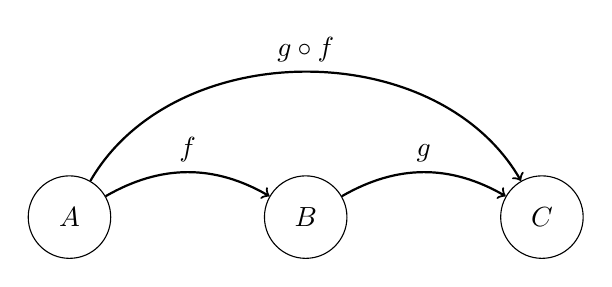
\begin{tikzpicture}
% Sets
    \node[draw, circle, text width=20pt,align=center] (A) at (0,0) {\(A\)};
    \node[draw, circle, text width=20pt,align=center] (B) at (3,0) {\(B\)};
    \node[draw, circle, text width=20pt,align=center] (C) at (6,0) {\(C\)};
% Functions
    \draw[->,thick] (A) to[bend left] node[pos=0.5,above] {\(f\)} (B);
    \draw[->,thick] (B) to[bend left] node[pos=0.5,above] {\(g\)} (C);
    \draw[->,thick,bend angle=60] (A) to[bend left] node[pos=0.5,above] {\(g\circ f\)} (C);
\end{tikzpicture}
